\chapter{INTRODUCTION}
Evolution has been intensively studied since the publication of \emph{On the Origin of Species} in order to untie the mysteries behind fascinating machineries within living systems. In a broader sense, most of the studies on evolutionary biology have two main goals: (I) To document history of life through evolutionary point of view, and (2) to understand causal mechanisms responsible for the biological diversity that we have on Earth \cite{futuyma2001evolution, hird2017evolutionary}. In addition to these goals, the idea of using pre-existing living systems as cell factories for industrial purposes gained close attention in the last decades \cite{nielsen2016engineering}.

Evolutionary engineering studies, adaptive laboratory evolution in particular, refers to the experiments in which the environmental conditions are altered gradually to obtain adapted populations in the laboratories \cite{garland2009experimental}. Accumulation of mutations obtained due to environmental alterations through generations, where the favored individuals (mainly the ones with increased fitness) are selected to become parents of the next generation, result a population with advantageous traits compared to starting population. Since one of the main challenges in the evolutionary engineering field is being able to analyze experimental to answer fundamental questions, adaptive evolution studies usually require interdisciplinary research in order to answer fundamental questions. What has changed in the cells through generations? What are the genetic basis for adaptation? Can we evolve any organism to any condition? If so, how? These questions and many more are asked everyday, and the corresponding answers potentially give rise to more questions.

The purpose of this thesis is to enlighten metabolic changes in the adaptation of the yeast \emph{S. cerevisiae} using computational methods, specifically genome-scale metabolic models. Evolved yeast strains (such as ethanol tolerant, long-lived, multi-stress resistant strains) are going to be analyzed comparetively to the unevolved strains using intracellular flux distributions obtained with the integration of transcriptomics data. This study will also contribute to the global understanding of metabolic regulations in yeast, and will be further expandable into metabolic engineering studies.

\chapter{THEORETICAL BACKGROUND}

\section{Adaptive Laboratory Evolution}
Since the very first laboratory evolution experiment was published in the late 19th century by William Dallinger, technological advancements allowed researchers to employ fully-controlled experiments for strain engineering to achieve desired traits \cite{dragosits2013adaptive}. Challenges in the experimental design of evolutionary studies, such as maintenance of the generations, controlling the environment, and feasibility to perform data analysis make the use of microorganisms in evolutionary studies more suited, especially \emph{Escherichia coli} and \emph{Saccharomyces cerevisiae} given their extensive characterization \cite{mcdonald2019microbial}.

Commonly used approaches of adaptive laboratory evolution (ALE) includes chemostat cultures and serial batch or colony transfers (Figure \ref{fig:ale}). Serial transfer experiments in which the initial population is aliquoted and transferred into a new medium are simpler and cheaper to set up, however the possibility of genetic drift is higher due to random sampling of the population. On the other hand, continuous systems such as chemostat experiments in bioreactors have advantages on maintaining constant growth rates and population sizes, but with increasing experimental cost \cite{winkler2013adaptive}.

\begin{figure}[ht]
\begin{center}
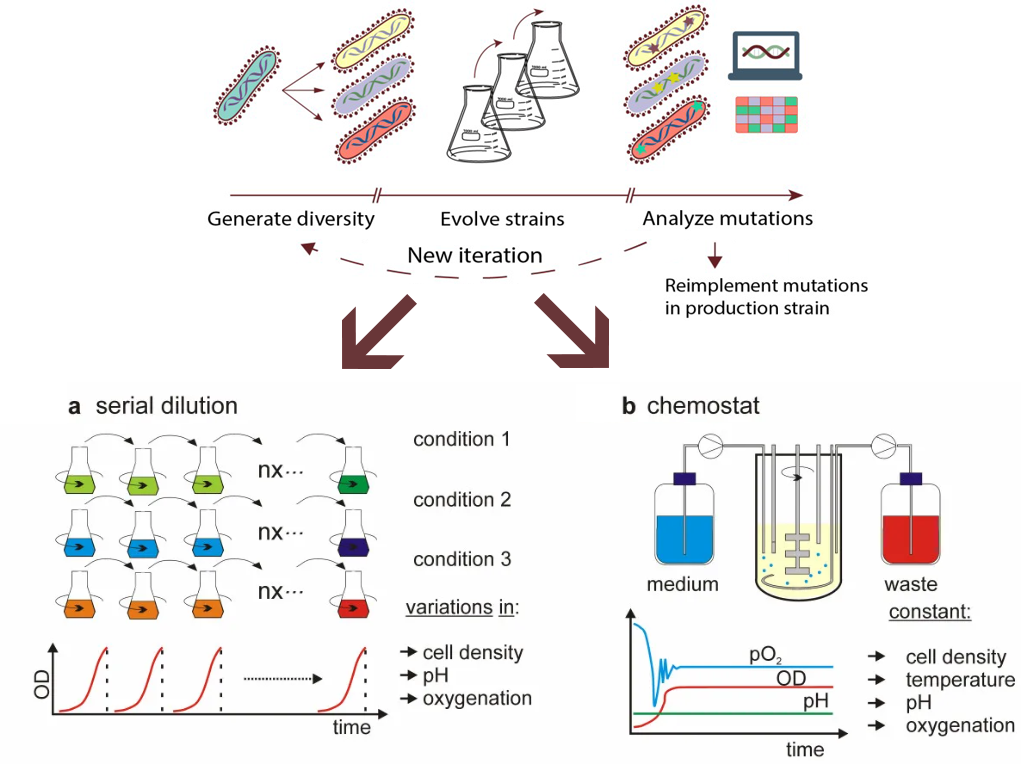
\includegraphics[width=1\columnwidth]{ALE.png}
\end{center}
\caption[Adaptive laboratory evolution workflow]{ALE methods and workflow. Figure is taken from \cite{dragosits2013adaptive} and \cite{shepelin2018selecting} and will be redrawn altogether.}
\vskip\baselineskip % Leave a vertical skip below the figure
\label{fig:ale}
\end{figure}

In addition to the methodological choice, decision of the selection criteria and the time span for the experiments are critical factors in ALE \cite{dragosits2013adaptive}. Growth rates, survivability in stressful environmental conditions and biomass yields are the most common fitness criteria for a population to be selected. Throughout the selection process, reaching \textgreater 500 generations may take a few weeks or a few months depending on the organism, therefore, detailed planning is essential \cite{conrad2011microbial}.

Capturing genomic changes in the dynamic evolution process is the main goal of an ALE study, therefore frequent data collection in longitudinal manner is a must to unveil molecular details. Next-generation technologies empower researchers to catch even single-nucleotide mutations through genome sequencing and also provide an understanding on broader regulatory changes through gene expression profiles \cite{conrad2011microbial}. Focus of the studying the differences between evolved and unevolved strains may be on the individual protein level or as a system-level trait. Interpreting the system as a network enables verious ways to investigate causality behind adaptive mechanisms and dynamics of evolution \cite{soyer2013evolutionary, long2018adaptive}.

\section{Systems Biology}
With the increasing availability of the computational tools and the development of high throughput techniques in the omics field, systems biology has shown a strong emergence in the last few years as a key multi-disciplinary field for integrating the multi-layer complexity of biological systems, particularly in the areas of transcriptomics, proteomics, metabolomics and fluxomics \cite{kitano2002systems}. This amount of available data allows researchers to investigate molecular cell processes in a large scales, applying theoretical, experimental and computational methods.

Biological systems based on complex interactions between various molecular components. The relations between these components are often obey nonlinear kinetics, for example, most of the reactions are regulated by one or more feedback or feed-forward loops with incomprehensible behaviours. When considered, cell structure and compartmentalization are also often introduce complexities to the unexpected behavior of the entire biological system \cite{bellouquid2006mathematical}. Mathematical modeling with these factors taken into consideration is used as a general approach to encompass existing knowledge in biological systems, and to gather information by analyzing these models to acquire a better understanding \cite{kremling2013systems}.

A mathematical model of a cell can be approached by two different approaches in either a bottom-up or top-down directionality (Figure \ref{fig:systemsbiology}) \cite{bruggeman2007nature, shahzad2012application}. Top-down approach is an experimental oriented approach, it starts from the whole picture and aims to characterize biological mechanisms closer to the smaller parts and their interactions in the network. In the bottom-up approach, collected data from biological knowledge is used as a starting point, a subsystem is generated to deduce the functional properties of smaller points in the network. Combination of the pathway level models (bottom-up) into a model for the entire system level (top-down) is the ultimate goal in the systems biology therefore these approaches are complementary.

\begin{figure}[ht]
\begin{center}
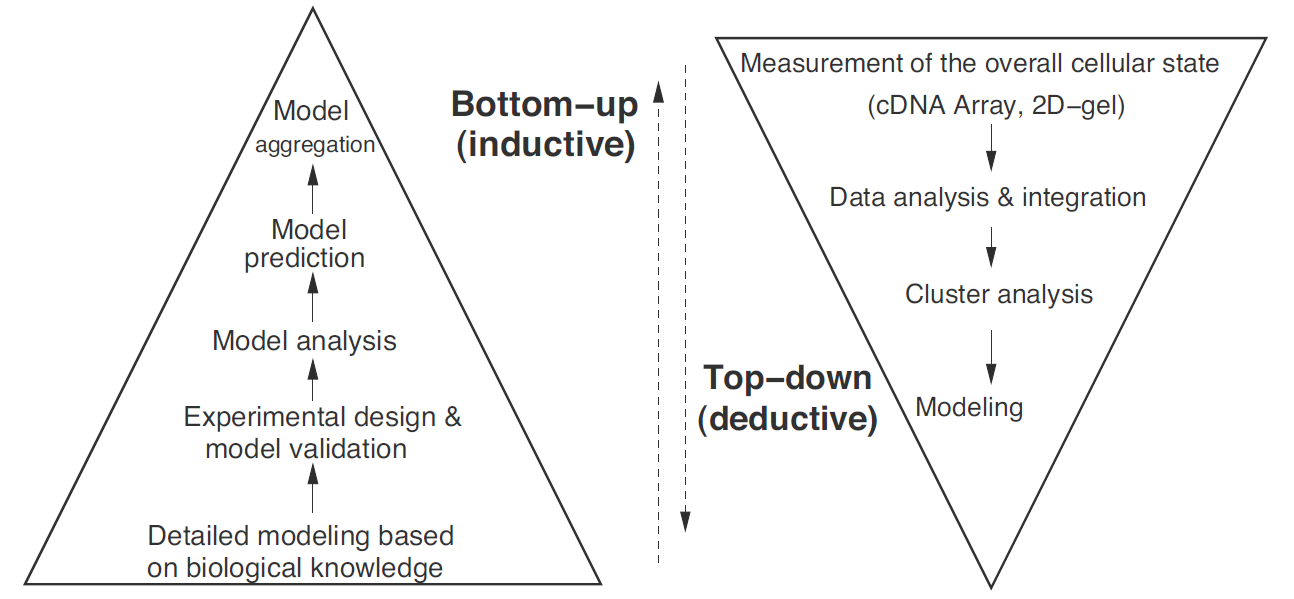
\includegraphics[width=0.8\columnwidth]{systemsbiology.png}
\end{center}
\caption[Systems biology approaches]{Systems biology approaches. Left: Bottom-up approach. Right: Top-down approach. Figure is taken from \cite{kremling2013systems}.}
\vskip\baselineskip % Leave a vertical skip below the figure
\label{fig:systemsbiology}
\end{figure}

\subsection{Metabolic Networks}
In the context of systems biology, metabolic network reconstructions have become a common interest for the researchers over the past 20 years \cite{thiele2010protocol}. Organism-specific metabolic network analyses allow scientists to design experiments and even obtain beforehand predictions. These networks are the main sources of the mathematical models which can simulate metabolic fluxes reflecting the experimantal reality \cite{orth2010flux}.

Before the improvement of genome sequencing or annotation technologies, initial core metabolic networks were based on the accessible information of biochemical pathways \cite{vallino1994carbon} \cite{varma1993biochemical}. In the last decade, larger genome-scale metabolic models (GSMMs) have been able to be developed rapidly with the help of databases for annotated genomes, providing information on substrates and products of each enzyme and each bioreaction \cite{feist2009reconstruction}. Growing biochemical databases provide automatization processes for the metabolic network reconstructions. As a result, genome-scale metabolic networks are available today for almost all organisms with an annotated genome available in the literature \cite{pitkanen2014comparative, kerkhoven2014applications}. From the first genome-scale metabolic model of \emph{Escherichia coli} to other organisms, the steps are required for GSMM development remained the same regardless of the biological diversity.

A generally applicable protocol is defined by the Palsson group \cite{thiele2010protocol, feist2009reconstruction} for the reconstruction of biochemical networks described in the Figure \ref{fig:modelreconstruction} \cite{chen2012metabolic}. Briefly, genomic data for the biochemical reactions of an organism are identified from the databases, such as NCBI, DDBJ and EMBL-EBI. Extraction and processing of the gene-protein-reaction relationship (GPR) of the genomic data results a draft reconstruction. GPR associations in the draft model should be reviewed by the researchers and manually curated if the identifying process is achieved with the help of automated computational algorithms \cite{pitkanen2014comparative}. Since the genomic data is the least representative of the biological phenotypes, available transcriptomic, proteomic, metabolomic and/or subcellular localization data are also used to further curate the model. Once the final metabolic network is reconstructed with bibliographic information, it is translated into a mathematical model.

\begin{figure}[ht]
\begin{center}
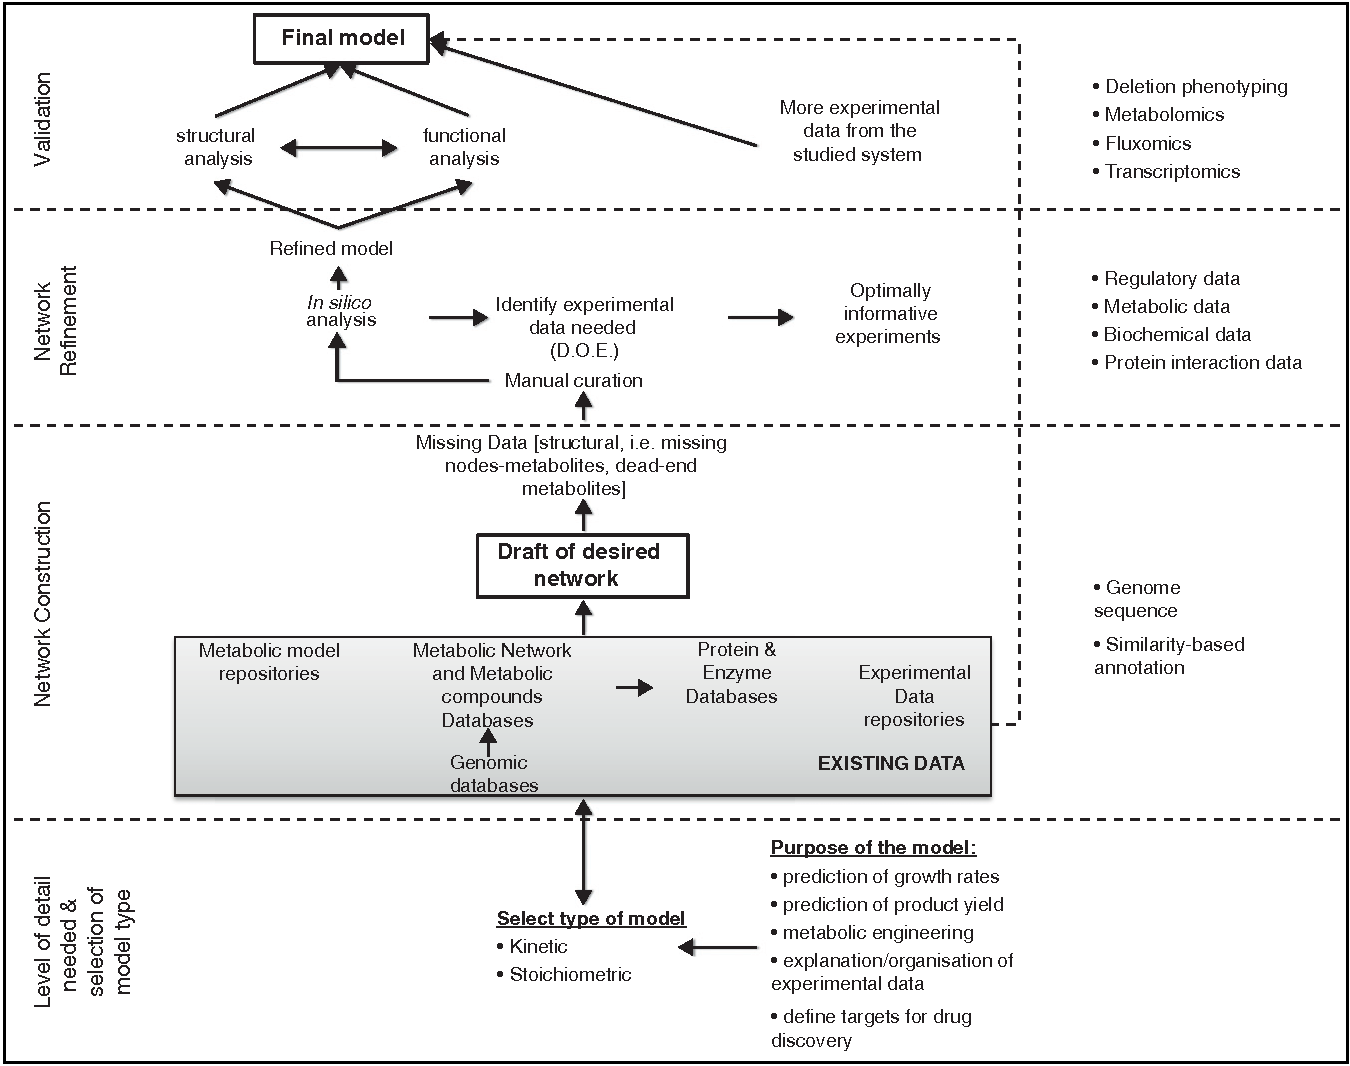
\includegraphics[width=1\columnwidth]{modelreconstruction.png}
\end{center}
\caption[Overview of metabolic network reconstruction protocol]{Overview of metabolic network reconstruction protocol. Figure is taken from \cite{chen2012metabolic}.}
\vskip\baselineskip % Leave a vertical skip below the figure
\label{fig:modelreconstruction}
\end{figure}

Once a metabolic network is reconstructed, a rational link between a genome sequence, the proteins encoded in the genome, and the reactions catalyzed by the proteins allowing to investigate the relationships between genotype and phenotype is achieved \cite{durot2008genome}. As the final step, GSMM needs to be validated by the new experimental data sets. GSMM validation process for various experimental conditions require detailed cultivation data from experiments. For example, information on the biomass composition of the specific organism leads more accurate biomass equation in the model, that is one of the key factors in the GSMM optimization and validation \cite{dikicioglu2015biomass}. Even tough multiple steps in the GSMM reconstruction can be achieved with the automated softwares available, it is usually necessary to curate the obtained model manually.

Approaches for analyzing metabolic networks are mainly categorized as dynamic or structural approaches. Even though the former is promising more realistic approach, its implementation in the literature is obstructed due to the unavailability of kinetic parameters for the majority of enzymes within a metabolic network \cite{machado2014systematic, ramkrishna2012dynamic} Because of the lack of kinetic parameters, structural metabolic modeling has been widely used for analyzing cellular metabolism at a steady-state assumption as a kind of snapshots taken at specific times.

GSMMs are one of the most useful tools in systems biology, especially in metabolic engineering studies \cite{kim2012recent}. In 1998, with the publication of \emph{Metabolic Engineering: Principles and Methodologies}, the term metabolic engineering is defined as the optimization of natural processes within cells to increase the production of certain substances \cite{stephanopoulos1999metabolic}. Hence, studies of metabolic engineering can be considered as genetic engineering in strain development. However, while metabolic engineering manipulates strains by altering flux distributions in the pathways; genetic engineering modificates specific genes, proteins and/or enzymes of interest \cite{stephanopoulos2012synthetic}. Although GSMMs are mainly used in metabolic engineering strategies, other applications both for descriptive and predictive purposes can be found in the literature \cite{osterlund2012fifteen}.

The ultimate goal of the GSMM reconstruction is to predict flux distribution profiles as close \emph{in silico} as they are \emph{in vivo}. Hence, GSMMs are in continuous research to improve predictability of organism-specific models.

\begin{figure}[ht]
\begin{center}
% 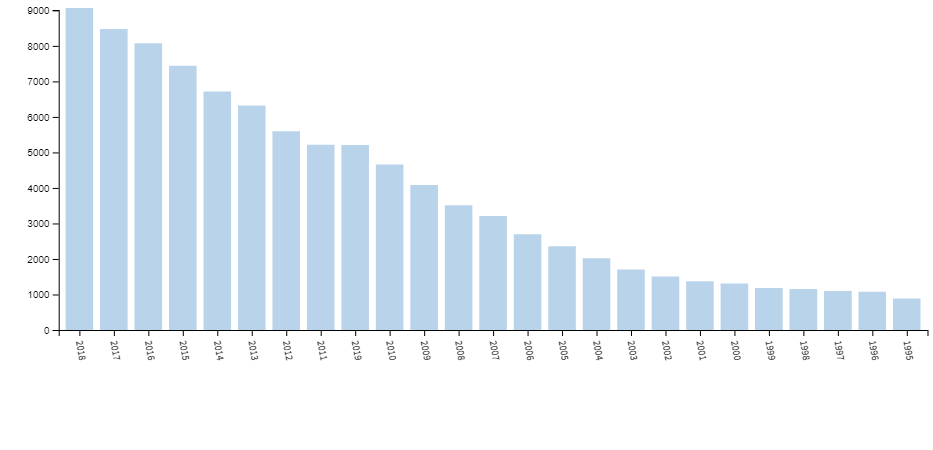
\includegraphics[width=1\columnwidth]{wos_metabolicmodel_search.jpg}
\end{center}
\caption[Web of Science artice counts on "metabolic model"]{Web of Science artice counts on "metabolic model"}
\label{fig:wos_metabolicmodel}
\end{figure}

\subsection{Mathematical Representation of Metabolic Networks}
Basic applications of metabolic network modelling, although its framework is developed by engineers or mathematicians, is used by biologists with various mathematical backgrounds \cite{pinzon2018mathematical}. In order to speak with one voice, fundamental concepts of mathematical representation of metabolic networks in GSMM reconstructions will be provided in this section.

One can propose a steady-state model for the correlation between the metabolites exist in the network. This model claims that the production and consumption of a metabolites must balance each other \cite{reimers2016steady}. For example, consider the metabolite "A" in the toy network in Figure \ref{fig:ToyNetwork}. It can be taken into cell with the rate of b1, and can be converted into B or C with the rates of v1 and v2 respectively; at the same time, metabolite C can be converted into A with the rate of v3. Note that enzyme kinetics are not considered and these equations are formed only considering mass balances.

\begin{figure}[h]
\begin{center}

\includegraphics[width=1\columnwidth]{ToyNetwork.png}
\end{center}
\caption[Toy network for steady-state assumption]{Toy network for steady-state assumption (will be redrawn).}
\label{fig:ToyNetwork}
\end{figure}

If we accept the steady-state assumption, and since we know all the possible reactions passing through metabolite A, we can write following differential equation

d(A)/dt = - v1 - v2 + v3 + b1 = 0

meaning that production rate of metabolite A is equal to its consumption rate. In other words, there will be no accumulation of metabolite A in the cell. Considering we have 3 metabolites and 7 reactions, this representation of reactions can written as a system of linear equations:
\begin{figure}[h]
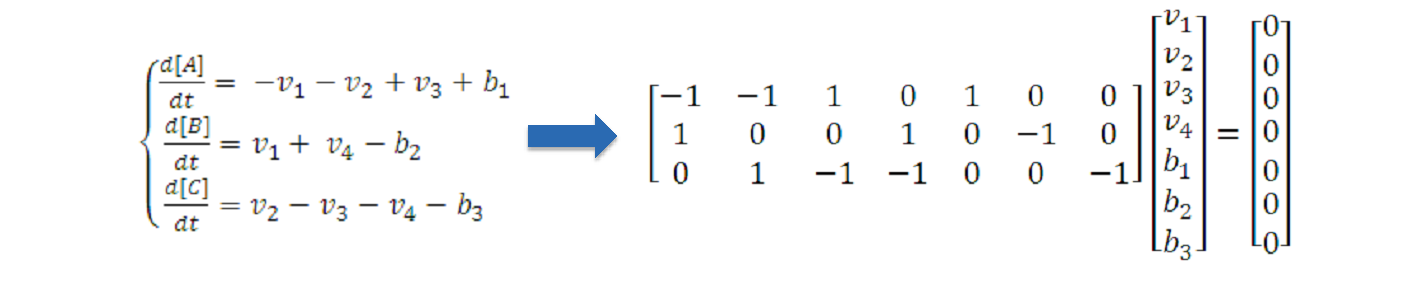
\includegraphics[width=1\columnwidth]{ToyNetworkEquations.png}
\begin{center}S . v = 0 \end{center}
\end{figure}

In the above equation, a matrix "S" appears. S matrix consists of stoichiometric coefficients of the reactions A single column of S matrix, representing a single reaction, provides information about the connections between the metabolites participating in that reaction; and a single row of S matrix, representing a metabolite, provides information about the connection of all the reactions in which that metabolite participates.

Next to S matrix a vector "v" appears. Vector "v" is called the flux vector, and it contains the change in concentration of metabolites. In other words, flux vector represents the flow rates or "fluxes" of each metabolite over time.

The solution space of S matrix, in the steady-state assumption, is generated by the null space base vectors of S. Studying on the null space vectors, we can define dead-end reactions (zero rows which mean reactions cannot carry flux), enzyme subsets (rows of scalar multiplies of each other, possibly chain reactions) and independent components (diagonal block structures in the null space, reactions that are independed from the network). Due to the large number of reactions in biological networks, the system is underdetermined and have multiple solutions in a convex flux cone space, referring to multiple steady-states of the cell.

\subsection{Constraint-Based Modeling}
As explained in the previous section, solution of a the metabolic network is not unique, meaning the model can be found in multiple states of flux distributions. In order to obtain more biologically relavant solutions, v vector can be constrained. \cite{thiele2007bringing}.


Cellular functions are limited by different types of constraints, which can be grouped in four general categories: fundamental physicochemical, spatial or topological, condition-dependent environmental, and regulatory or self-imposed constraints. Although the first two categories of constraints are assumed to be independent from the environment, the latter two may vary in the simulation.


\section{\emph{Saccharomyces cerevisiae}}

The species "yeast" includes a range of eukaryotic single-celled microorganisms, although it is commonly used to describe \emph{Saccharomyces cerevisiae}. Also known as the baker's yeast, \emph{S. cerevisiae} is one of the extensively used microorganisms for alcoholic fermentation of beverages, bio-ethanol production, and processing various foods since ancient times \cite{gelinas2009inventions}. It was the first eukaryotic organism whose genome was fully sequenced and annotated \cite{goffeau1997multidrug}, and besides its benefits in the industry, it is used as a model system for other eukaryotic cells including humans \cite{dujon1996yeast, botstein1997yeast}.

\subsection{Central Carbon Metabolism of \emph{S. cerevisiae}}
From the end of the eighteenth century, mainly after the fermentation is defined as "respiration without oxygen", the metabolism of \emph{S. cerevisiae} has been studied extensively \cite{barnett1998history, barnett2000history}. Its capability to produce ethanol is one of the most characterized microbial processes due to industrial utilization.

The set of anabolic and catabolic reactions in the cell are reffered as the metabolism. A shematic representation of the central carbon metabolism in \emph{S. cerevisiae} can be found in Figure \ref{fig:central_carbon_mech_of_s_cerevisiae_kegg}. Glycolysis, pentose-phosphate pathway (PPP), tricarboxylic acid cycle (TCA) or Krebs cycle, the glyoxylate cycle and the electron transport chain are the main pathways in central carbon metabolism.

 \begin{figure}[ht]
 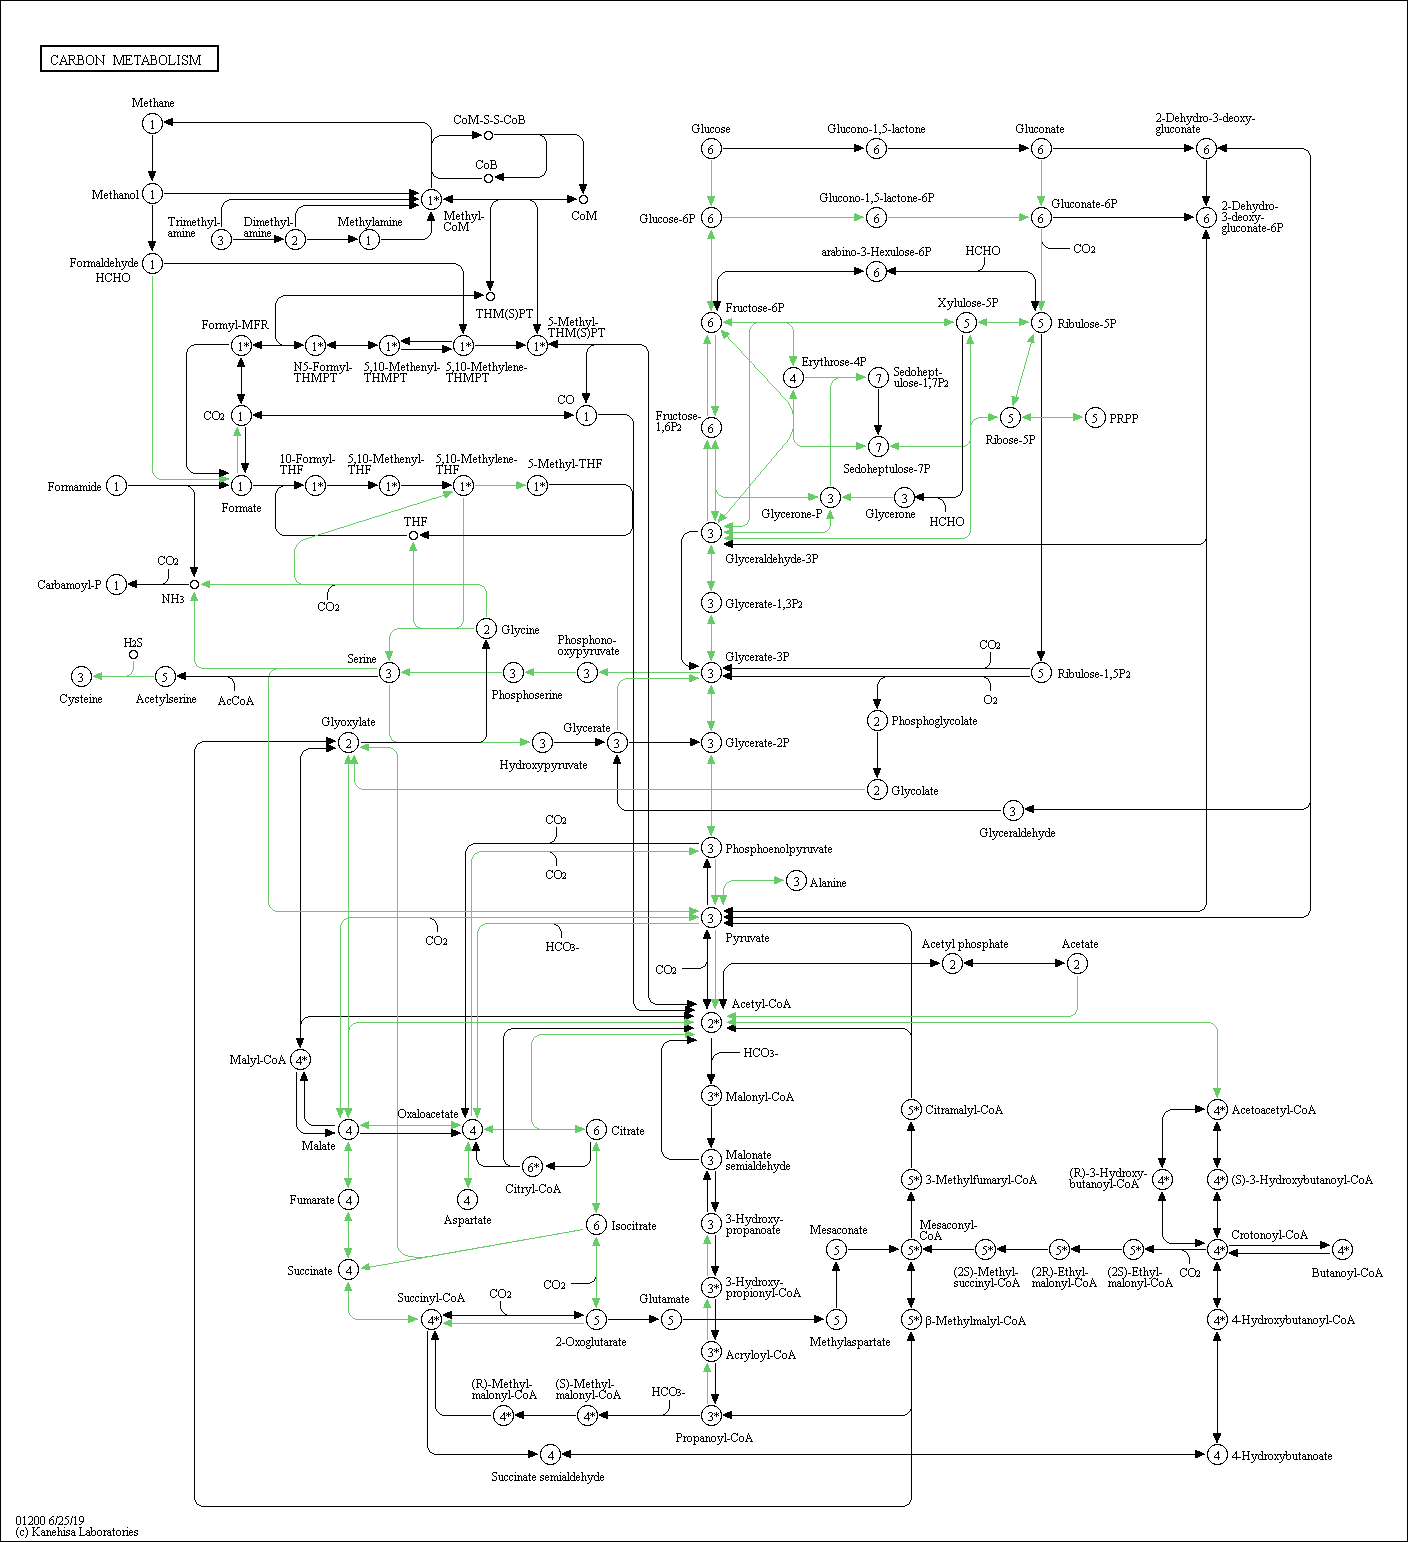
\includegraphics[width=1\columnwidth]{central_carbon_mech_of_s_cerevisiae_kegg.png}
 \caption[Central carbon mechanism of \emph{S. cerevisiae}]{Central carbon mechanism of \emph{S. cerevisiae} obtained from  KEGG \cite{kanehisa2000kegg}.}
 \vskip\baselineskip % Leave a vertical skip below the figure
 \label{fig:central_carbon_mech_of_s_cerevisiae_kegg}
 \end{figure}

\hl{In this section, there will be subsections on} all biological pathways individually (explaining each in detail -probably referencing Lehninger biochemistry-) especially NAD regulation, fermantation (crabtree effect, industrial applications, bio-ethanol production) etc... Maybe also regulation strategies in cells (feedback/feedforward loops with figures)

\subsection{Adaptive Evolution Studies on \emph{S. cerevisiae} (Palsson 2015)}

\subsection{Metabolic Models of \emph{S. cerevisiae}}
After the first \emph{S. cerevisiae} genome sequence is published, the first cDNA spotted microarray exploring metabolic gene regulation in 1997 \cite{derisi1997exploring}, and the first commercial platform for oligonucleotide microarray data (Affymetrix) to investigate cellular regulations were reported in 1998 \cite{cho1998parallel}. Existing genome data is integrated with the extensive annotation based on microarray data and biochemical knowledge from literature, leading of the publication of the first GSMM of \emph{S. cerevisiae} in 2013 \cite{forster2003genome}.   \hl{More in this section, there will be review on:} Genome-scale modeling of yeast: chronology, applications and critical perspectives \cite{lopes2017genome}

\subsection{Applications of \emph{S. cerevisiae} GSMMs}
 \hl{Literature review on the applications will be added.}
